\section*{Back Up}

\begin{frame}{}
% \thispagestyle{empty}
\centering	\Huge{\textbf{BACK UP}}
\end{frame}

\begin{frame}{Probability Weighting as an Estimation Issue}
\textquote[{\cite[281]{KahnemanTversky1979}}]{It is important to distinguish \blue{overweighting}, which refers to a property of decision weights, from the \blue{overestimation} that is commonly found in the assessment of the probability of rare events.
[...]
% Note that the issue of overestimation does not arise in the present context, where the subject is assumed to adopt the stated value of $p$.
In many real-life situations, overestimation and overweighting may both operate to increase the impact of rare events.}

\vspace{1em}

\bi
	\item[$\hookrightarrow$] distinguish between
	\bi
		\item uncertainty estimation and
		\item \textquote{weighting}
	\ei
	we analyse the former and find very good agreement with the empirical inverse-S pattern
	\item[$\hookrightarrow$] How big is the residual \textquote{probability weighting} after accounting for uncertainty estimation?
\ei
% has the same effect on human decisions as probability weighting. Since they assumed that subjects in experiments adopt unquestioningly the stated probabilities, they argued that probability weighting was necessary to explain their observations. We make no such assumption here.
\vfill
\label{weight_vs_estimate}
\hyperlink{MainResults}{\beamerreturnbutton{Main Results}}
\end{frame}

\begin{frame}{Estimation Error Explains 99\% of Probability Weighting}
\bc
	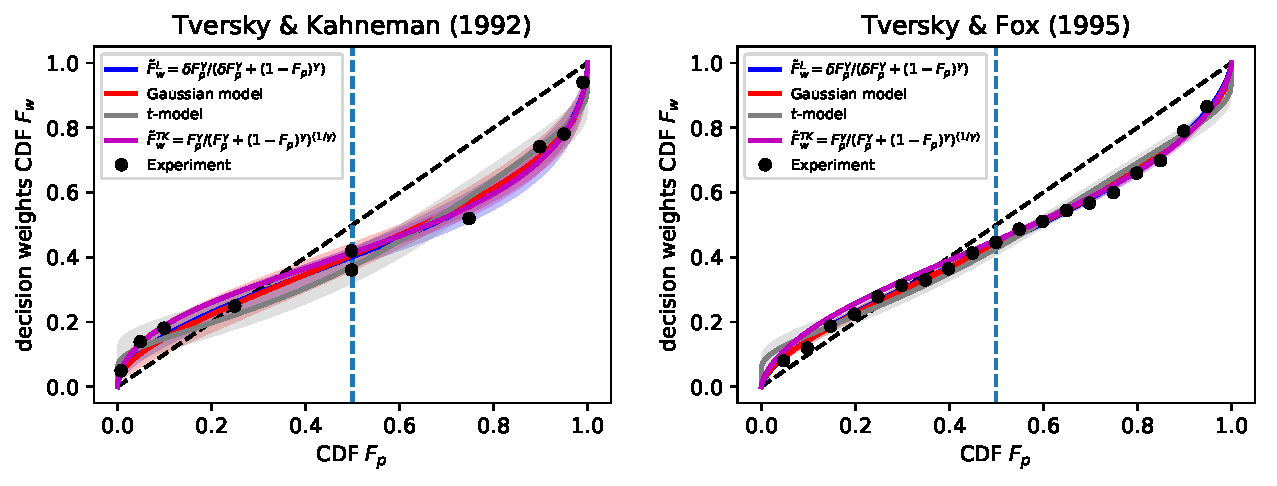
\includegraphics[width=\textwidth]{../../figs/curvefit}
\ec

% \vspace{1em}

\bi
	\item	similar fits of Gaussian \& $t$-distributed model% with the empirical inverse-S pattern
	\item[$\hookrightarrow$] How big is the residual \textquote{probability weighting} after accounting for  estimation errors?
\ei
\hyperlink{MainResults}{\beamerreturnbutton{Main Results}}

\end{frame}

\begin{frame}{Functional Forms
\hyperlink{InterimConclusion}{\beamerreturnbutton{Gaussian}}} \label{FunctionalForms}
\textcite[$\gamma = 0.68$]{TverskyKahneman1992}
\be \label{correspondence}
	\tilde{F}^{TK}_w\left(F_p; \gamma\right) = \left(F_p\right)^\gamma \frac{1}{\left[\left(F_p\right)^\gamma+\left(1-F_p\right)^\gamma\right]^{1/\gamma}}
\ee

\textcite{LattimoreBakerWitte1992}
\be \label{LattimoreFunction}
\tilde{F}^{L}_w\left(F_p; \delta,\gamma\right) =\frac{\delta F_p^{\gamma}}{\delta F_p^{\gamma} + \left(1-F_p\right)^{\gamma}}
\ee

Gaussian case with greater DM scale $\alpha \sigma$
\be \elabel{w_of_p}
w(p)= p^{\frac{1}{\alpha^2}} \frac{\left(2\pi\sigma^2\right)^{\frac{1-\alpha^2}{2\alpha^2}}}{\alpha} ~,
\ee
which is a power law in $p$ with a pre-factor to ensure normalisation
\end{frame}


% \begin{frame}{Linking Probability Weighting to Relative Uncertainties}
% Decision weight $w$ is the normalised sum of the probability $p(x)$ and its uncertainty $\err{p(x)}$
% \be
% 	w(x)=\frac{p(x)+\err{p(x)}}{\int_{-\infty}^{\infty} \left( p(s)+\err{p(s)} \right) ds}	~.
% \ee
% This can be expressed as
% \be
% w(x)=p(x) \left(\frac{1+\frac{\err{p(x)}}{p(x)}}{\int_{-\infty}^{\infty} p(s)\left\{1+\frac{\err{p(s)}}{p(s)}\right\} ds}\right)~,
% \label{rel_error}
% \ee
% where $\frac{\err{p(x)}}{p(x)}$ is the relative error, which is large (small) for small (large) probabilities
% 
% In the long-time limit $w(x) \to p(x)$
% \end{frame}
%  
